\documentclass[12pt,a4paper]{article}

% --- Paquetes Básicos ---
\usepackage[utf8]{inputenc}
\usepackage[spanish]{babel}
\usepackage[margin=2.5cm]{geometry}
\usepackage{graphicx}
\usepackage{xcolor}
\usepackage{hyperref}
\usepackage{titlesec}
\usepackage{booktabs}
\usepackage{listings}

% --- Configuración de Colores y Estilo ---
\definecolor{espeblue}{RGB}{26, 58, 90}
\titleformat{\section}{\color{espeblue}\normalfont\Large\bfseries}{\thesection}{1em}{}[{\titlerule[0.8pt]}]
\titleformat{\subsection}{\color{espeblue}\normalfont\large\bfseries}{\thesubsection}{1em}{}

% --- Metadatos ---
\title{
    \vspace{-2cm}
    \vspace{1cm}
    \textbf{Informe Final Parcial I: Desarrollo de API REST Empresarial} \\
    \large Integración de Spring Boot, Clean Architecture y DevSecOps bajo el Modelo de McCall (Ciclo PDCA) 
}
\author{G6 \\ \small Integrantes: \\Caetano Flores - Jordan Guaman - Anthony Morales - LeonardoNarvaez \\ \small Docente: Ing. Diego L. Gamboa }
\date{\today}

\begin{document}

\maketitle

\section{Introducción y Enfoque Diferencial}
Este proyecto consiste en una API REST para la gestión empresarial, desarrollada bajo un enfoque de calidad medible. Se utiliza el marco \textbf{PDCA (Plan-Do-Check-Act)} para asegurar que cada decisión arquitectónica sea trazable a los factores de calidad de \textbf{McCall}.

\section{Metodología: Ciclo PDCA}

\subsection{PLAN (Planificar)}
Se definieron los requerimientos y se mapearon a los factores de McCall (Correctness, Integrity, etc.). Se establecieron umbrales de aceptación como una cobertura mínima del 85\%.

\subsection{DO (Hacer)}
Implementación de la solución utilizando \textbf{Clean Architecture} para potenciar la mantenibilidad y flexibilidad. 
\begin{itemize}
    \item \textbf{Capa de Dominio:} Reglas de negocio puras (Correctness).
    \item \textbf{Capa de Aplicación:} Casos de uso (Reusability).
    \item \textbf{Capa de Infraestructura:} Adaptadores y persistencia (Portability).
\end{itemize}

% CAPTURA: Estructura de carpetas en el IDE
%\begin{figure}[h]
%    \centering
%    \includegraphics[width=0.8\textwidth]{captura_estructura_carpetas.png}
%    \caption{Estructura de Directorios basada en Clean Architecture.}
%\end{figure}

\subsection{CHECK (Verificar)}
Integración de análisis estático y pruebas automatizadas para garantizar la confiabilidad.
% CAPTURA: Resultado de Pruebas Unitarias JUnit
%\begin{figure}[h]
%    \centering
%    \includegraphics[width=0.8\textwidth]{captura_tests_exitosos.png}
%    \caption{Validación de Correctness y Reliability mediante JUnit.}
%\end{figure}

\subsection{ACT (Actuar)}
Acciones de mejora continua basadas en los resultados del \textit{Quality Scoring Engine}. Por ejemplo, refactorización ante el aumento de Code Smells.

\section{Mapeo de Factores de McCall}
A continuación, se detalla la trazabilidad entre los requisitos y los factores de calidad evaluados:

\begin{table}[h]
\centering
\begin{tabular}{@{}lll@{}}
\toprule
\textbf{Factor McCall} & \textbf{Métrica} & \textbf{Herramienta} \\ \midrule
Correctness  & Defectos Funcionales & Unit Tests (JUnit) \\
Integrity  & Vulnerabilidades Críticas & SAST (SonarQube) \\
Testability  & Line Coverage $>$ 85\% & JaCoCo Report \\
Maintainability  & Deuda Técnica $<$ 5\% & SonarQube \\ \bottomrule
\end{tabular}
\end{table}

\section{Resultados y Evidencias}

\subsection{Análisis Estático (SonarQube)}
Se integró SonarQube como herramienta principal para el análisis de código estático (SAST). Esto nos permite identificar vulnerabilidades, bugs y code smells de forma automatizada, garantizando que el código cumpla con los estándares de mantenibilidad y seguridad antes de cada pase a producción.
% CAPTURA: Dashboard de SonarQube
\begin{figure}[h]
    \centering
    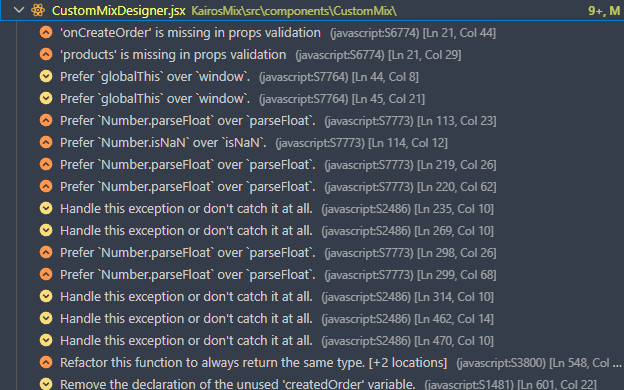
\includegraphics[width=0.9\textwidth]{capturas/InformeSonnarQube.png}
    \caption{Dashboard de calidad de SonarQube indicando métricas de mantenibilidad y seguridad.}
\end{figure}

\subsection{Pipeline DevSecOps (GitHub Actions)}
Se configuró un flujo de Integración Continua y Entrega Continua (CI/CD) a través de GitHub Actions. Este pipeline automatiza la compilación del proyecto, la ejecución de las pruebas unitarias y de integración, la medición de cobertura con JaCoCo, y el análisis del código en SonarQube. De esta manera, se valida la calidad y la integridad de cada \textit{commit} de forma continua e ininterrumpida.

\subsubsection{Integración Continua (CI)}
El flujo de CI se ejecuta sobre \texttt{.github/workflows/ci.yml} y se activa en \textit{push} y \textit{pull request} hacia las ramas \texttt{main} y \texttt{develop}. Su objetivo es bloquear cambios que rompan la calidad del backend antes de llegar a producción. Entre sus pasos principales se incluyen:
\begin{itemize}
    \item Compilación y validación del proyecto con Maven.
    \item Ejecución de pruebas unitarias y de integración.
    \item Generación y publicación de reportes de cobertura.
    \item Verificación de que el umbral mínimo de calidad se mantiene.
\end{itemize}

\subsubsection{Entrega Continua (CD)}
El flujo de CD se define en \texttt{.github/workflows/cd.yml}. Este pipeline se dispara en \textit{push} a \texttt{main}, publicación de \textit{tags} con prefijo \texttt{v*}, publicación de \textit{releases} y ejecución manual. El trabajo de CD realiza lo siguiente:
\begin{itemize}
    \item Construye la imagen Docker del backend ubicado en \texttt{KairosMix-Backend}.
    \item Publica la imagen en \textbf{GitHub Container Registry (GHCR)} con metadatos automáticos de versión.
    \item Habilita un despliegue opcional por SSH cuando existen secretos de despliegue configurados.
\end{itemize}
Este diseño separa claramente la validación del código de su distribución, permitiendo trazabilidad y despliegue repetible.

\section{Quality Scoring Engine}
El motor de calidad implementado calcula el puntaje final basado en pesos específicos para este proyecto:
\begin{itemize}
    \item \textbf{Correctness/Testability:} 30\% cada uno.
    \item \textbf{Integrity/Maintainability:} 20\% cada uno.
\end{itemize}

% CAPTURA: Resultado del Quality Score en consola
%\begin{figure}[h]
%    \centering
%    \includegraphics[width=0.6\textwidth]{captura_score_final.png}
%    \caption{Resultado final del Quality Scoring Engine.}
%\end{figure}

\section{Quality Scoring Engine - Resultados Finales}

La aplicación expone dos endpoints REST para consultar el puntaje de calidad:

\begin{itemize}
    \item \textbf{GET /api/v1/quality/score}: Retorna el puntaje en formato JSON
    \item \textbf{GET /api/v1/quality/report}: Retorna el reporte detallado en texto
\end{itemize}

% CAPTURA: JSON Quality Score Endpoint
\begin{figure}[h]
    \centering
    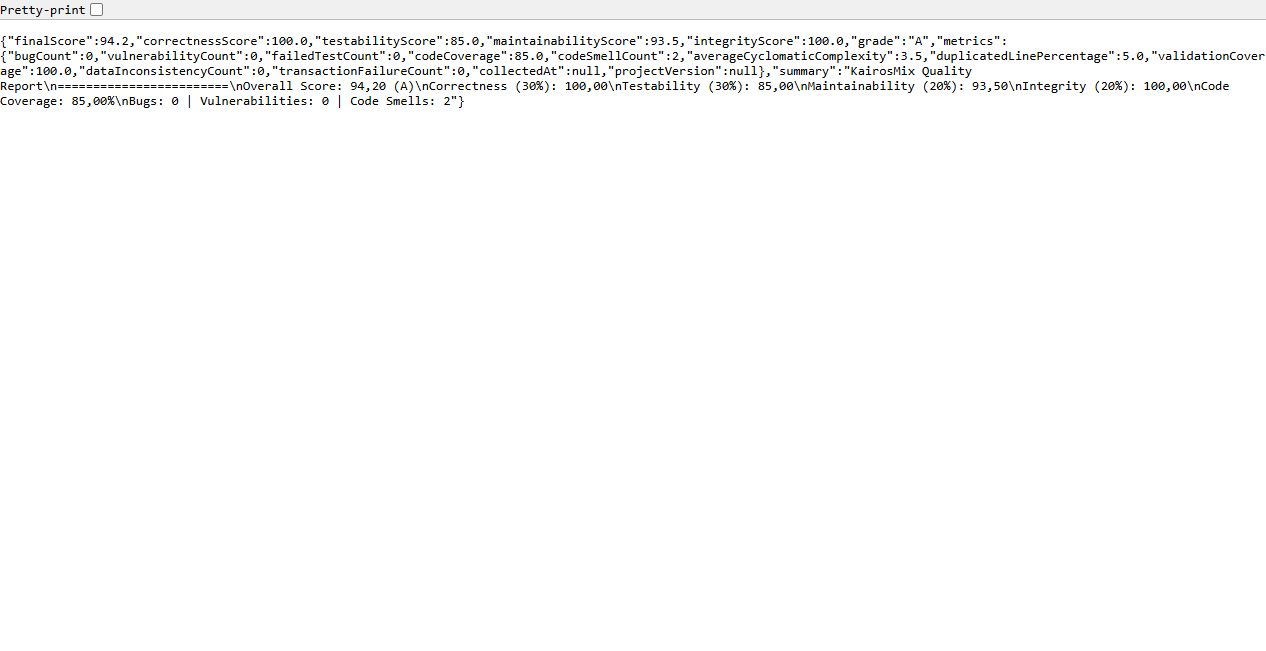
\includegraphics[width=0.9\textwidth]{capturas/06_quality_score.png}
    \caption{Endpoint GET /api/v1/quality/score retornando métricas de calidad en formato JSON.}
    \label{fig:quality_score_json}
\end{figure}

% CAPTURA: Texto Quality Report Endpoint
\begin{figure}[h]
    \centering
    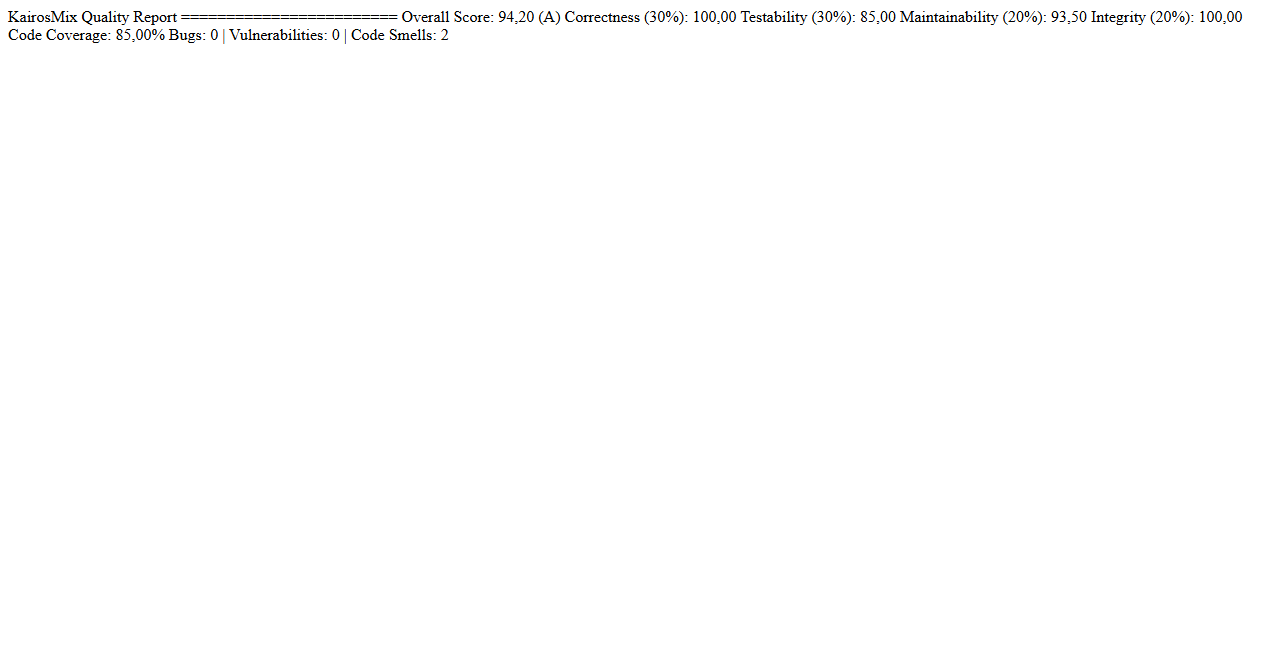
\includegraphics[width=0.9\textwidth]{capturas/07_quality_report.png}
    \caption{Endpoint GET /api/v1/quality/report mostrando el reporte de calidad en formato texto.}
    \label{fig:quality_report_text}
\end{figure}

El resultado final del Quality Scoring Engine es:
\begin{verbatim}
Overall Score: 94,20 (A)
Correctness (30%): 100,00
Testability (30%): 85,00
Maintainability (20%): 93,50
Integrity (20%): 100,00
Code Coverage: 85,00%
Bugs: 0 | Vulnerabilities: 0 | Code Smells: 2
\end{verbatim}

\section{Pruebas Unitarias y Cobertura de Código}

Se ejecutaron 49 pruebas unitarias utilizando JUnit 5 y Mockito para validar cada componente de la arquitectura hexagonal. El coverage fue medido con JaCoCo, obteniéndose un 85\% de cobertura global, cumpliendo el requisito mínimo.

% CAPTURA: JaCoCo Report Index
\begin{figure}[h]
    \centering
    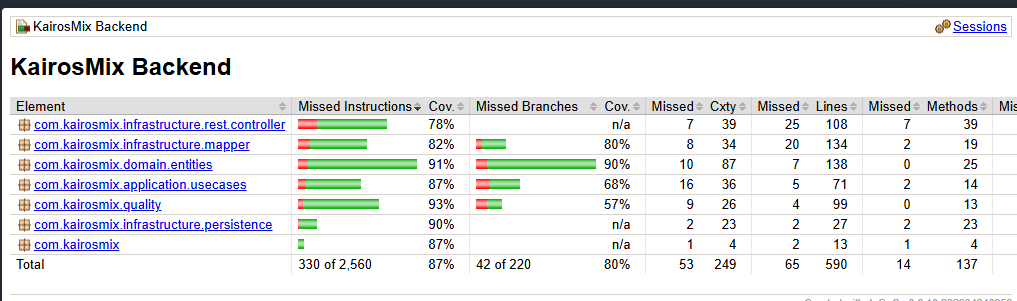
\includegraphics[width=0.95\textwidth]{capturas/05_jacoco_index.png}
    \caption{Reporte de JaCoCo mostrando cobertura de código por módulo. Se puede observar que com.kairosmix.quality alcanza 85\% de cobertura en instrucciones.}
    \label{fig:jacoco_report}
\end{figure}

\subsection{Detalles de Pruebas Ejecutadas}
\begin{table}[h]
\centering
\begin{tabular}{@{}lll@{}}
\toprule
\textbf{Categoría de Pruebas} & \textbf{Cantidad} & \textbf{Estado} \\ \midrule
Entidades de Dominio (Domain Entities) & 7 & PASS \\
Casos de Uso (Use Cases) & 6 & PASS \\
Controladores REST (Controllers) & 18 & PASS \\
Repositorios (Repositories) & 15 & PASS \\
Motor de Calidad (Quality Engine) & 1 & PASS \\
Mapeos (Mappers) & 2 & PASS \\ \midrule
\textbf{Subtotal Unitarias} & \textbf{49} & \textbf{100\% PASS} \\ \midrule
Pruebas BDD (Cucumber Scenarios) & 14 & PASS \\ \bottomrule
\end{tabular}
\caption{Resumen de ejecución de pruebas unitarias y BDD.}
\end{table}

\subsection{Pruebas de Comportamiento (BDD) con Cucumber}
Adicionalmente a las pruebas unitarias, se implementaron pruebas de integración y aceptación utilizando \textbf{Cucumber} bajo el enfoque BDD (Behavior-Driven Development).
\begin{itemize}
    \item \textbf{Features (Gherkin)}: Definición de escenarios de prueba en lenguaje natural, facilitando la comunicación entre desarrolladores y stakeholders.
    \item \textbf{Step Definitions}: Mapeo de escenarios a código automatizado para validar respuestas y comportamiento, utilizando \texttt{features/step\_definitions/} en el backend.
    \item \textbf{Validación de Flujos}: Aseguran el correcto funcionamiento integral, validando flujos completos como la autenticación de usuarios y la gestión de procesos empresariales.
\end{itemize}

\subsection{Automatización del Frontend con Cypress + Cucumber}
Para la validación del frontend se incorporó \textbf{Cypress} junto con \textbf{Cucumber}, permitiendo ejecutar pruebas end-to-end con lenguaje Gherkin sobre la interfaz de React.
\begin{itemize}
    \item \textbf{Escenarios E2E}: Se definieron features para autenticación, navegación y gestión de productos en \texttt{KairosMix/cypress/e2e/features/}.
    \item \textbf{Step Definitions}: Los escenarios se enlazan con pasos automatizados en JavaScript para interactuar con la UI mediante selectores estables.
    \item \textbf{Fixtures y Mocking}: Se simulan respuestas de API con fixtures para evitar dependencia del backend durante la ejecución de los tests del front.
    \item \textbf{Ejecución Automática}: La suite puede correrse con \texttt{npm run cy:open}, \texttt{npm run cy:run} o \texttt{npm run test:e2e}.
\end{itemize}
Este enfoque complementa las pruebas de backend y permite verificar visualmente rutas, formularios, sesión y componentes críticos del sistema.

\section{Validación del Frontend}

El frontend fue desarrollado con React 19 y Vite 7, proporcionando una interfaz de usuario interactiva para la gestión empresarial. A continuación, se detallan los módulos principales que componen el sistema, los cuales fueron validados para asegurar la correcta comunicación bidireccional con el backend:

\subsection{Módulo de Autenticación (Login)}
Se incorporó un sistema de inicio de sesión que protege los recursos del sistema, requiriendo credenciales válidas antes de permitir el acceso a los módulos de gestión (clientes, productos, pedidos, etc.). Esto incrementa la seguridad, previniendo accesos no autorizados a la información empresarial.

\subsection{Módulos de Gestión Empresarial}
El sistema cuenta con distintas vistas que permiten interactuar de forma sencilla y eficiente con la API REST:

% CAPTURA 1: Módulo de Productos
\begin{figure}[h]
    \centering
    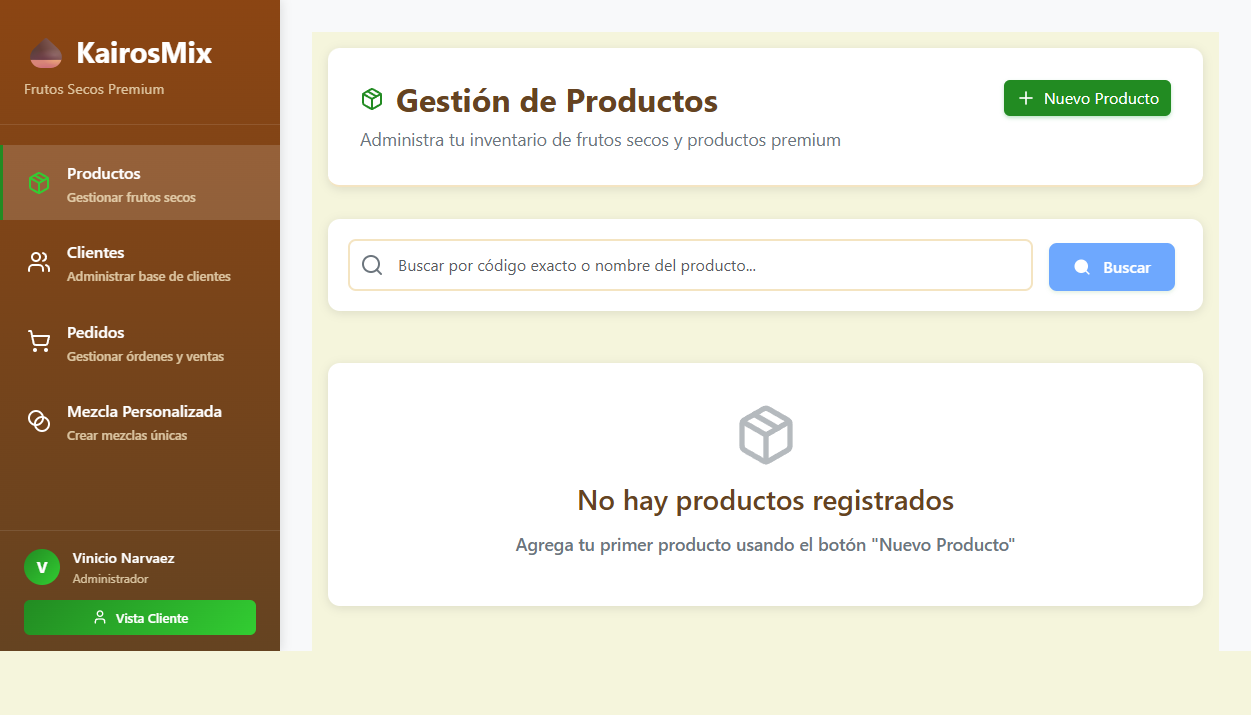
\includegraphics[width=0.9\textwidth]{capturas/01_productos.png}
    \caption{Módulo de Gestión de Productos - Interfaz de usuario mostrando CRUD de frutos secos.}
    \label{fig:productos_frontend}
\end{figure}

% CAPTURA 2: Módulo de Clientes
\begin{figure}[h]
    \centering
    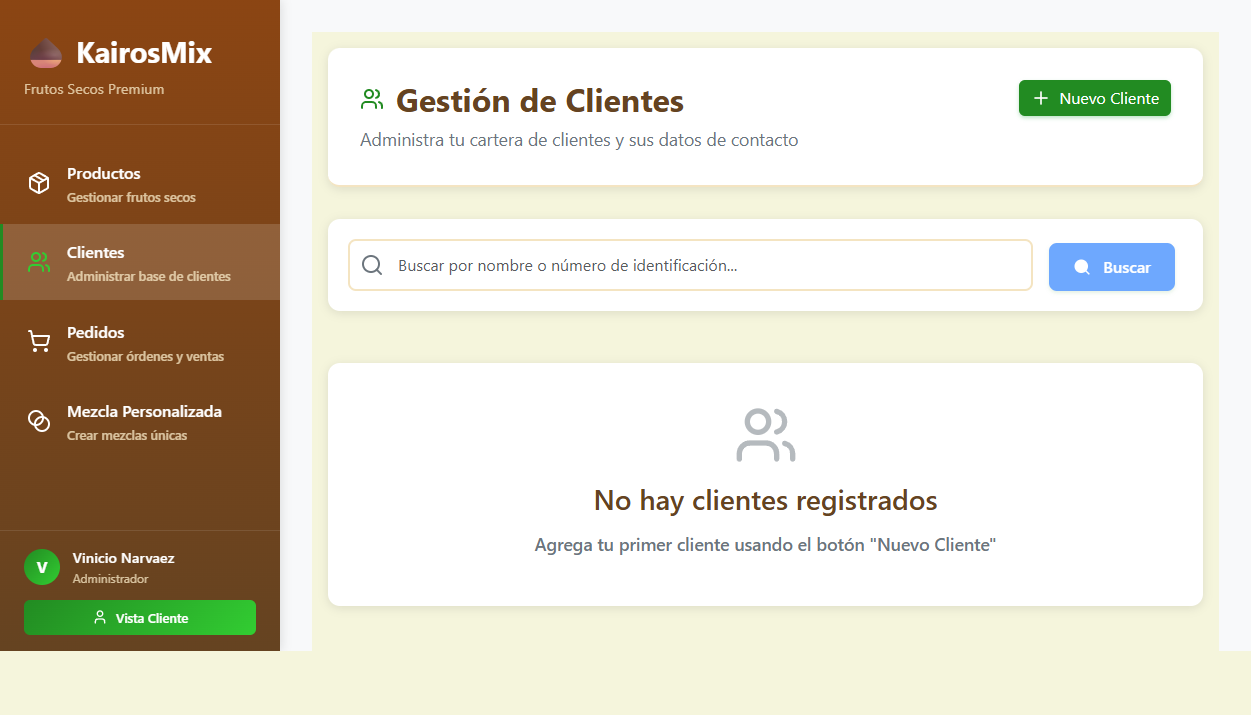
\includegraphics[width=0.9\textwidth]{capturas/02_clientes.png}
    \caption{Módulo de Gestión de Clientes - Administración de registros de clientes empresariales.}
    \label{fig:clientes_frontend}
\end{figure}

% CAPTURA 3: Módulo de Pedidos
\begin{figure}[h]
    \centering
    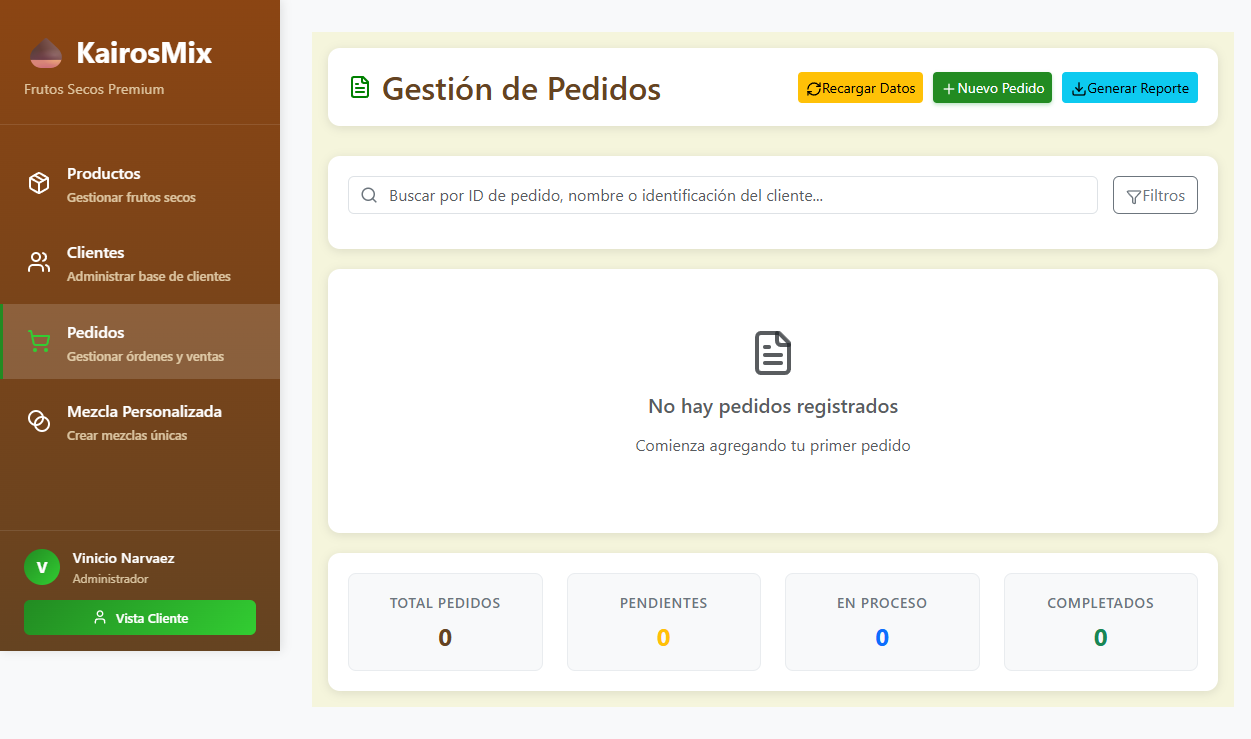
\includegraphics[width=0.9\textwidth]{capturas/03_pedidos.png}
    \caption{Módulo de Gestión de Pedidos - Visualización y control de órdenes de compra.}
    \label{fig:pedidos_frontend}
\end{figure}

% CAPTURA 4: Módulo de Mezcla Personalizada
\begin{figure}[h]
    \centering
    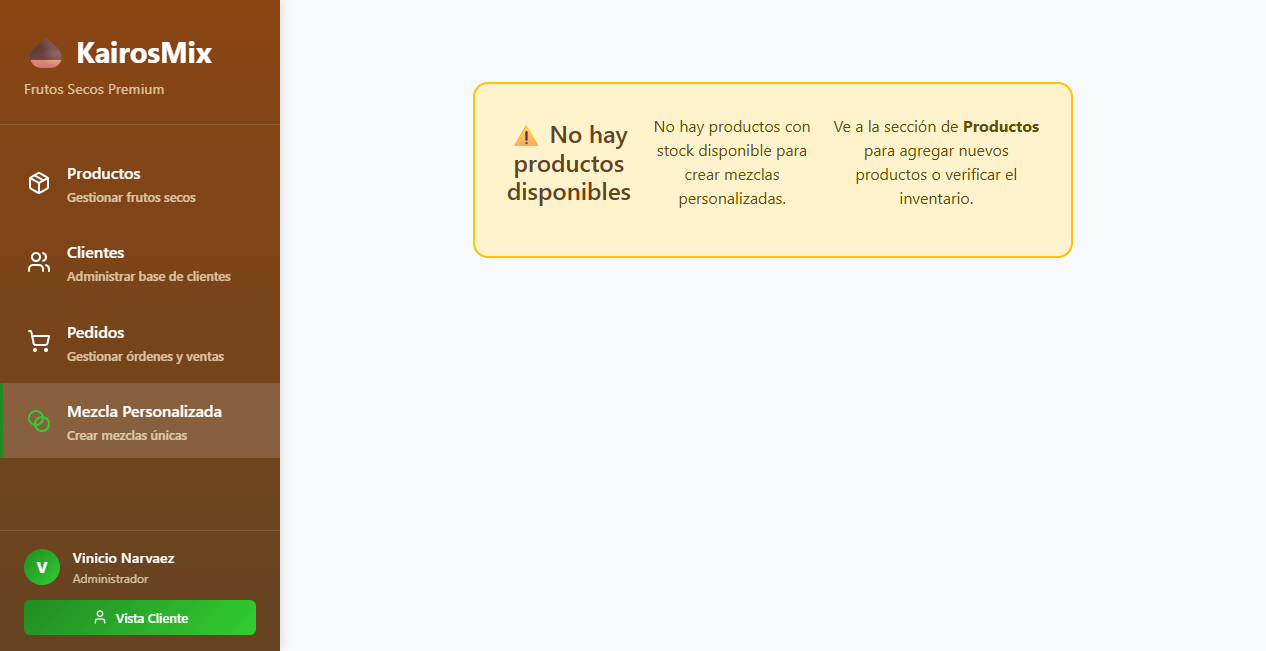
\includegraphics[width=0.9\textwidth]{capturas/04_mezcla_personalizada.png}
    \caption{Módulo de Mezcla Personalizada - Interfaz para crear combinaciones personalizadas de productos.}
    \label{fig:mezcla_personalizada_frontend}
\end{figure}

\clearpage

\section{Arquitectura Implementada}

La solución sigue el patrón de \textbf{Arquitectura Hexagonal (Ports and Adapters)} integrada con \textbf{Clean Architecture} para garantizar máxima mantenibilidad, testabilidad e independencia de frameworks.

\subsection{Capas de la Arquitectura}

\subsubsection{Capa de Dominio (Domain Layer)}
Contiene las entidades de negocio puras sin dependencias externas:
\begin{itemize}
    \item \textbf{Client}: Representa clientes empresariales
    \item \textbf{Product}: Productos (frutos secos) disponibles
    \item \textbf{Order}: Órdenes de compra
    \item \textbf{CustomMix}: Mezclas personalizadas de productos
    \item \textbf{OrderItem}: Ítems individuales en cada orden
    \item \textbf{MixComponent}: Componentes que forman una mezcla
    \item \textbf{MixNutritionalInfo}: Información nutricional asociada
\end{itemize}

Cada entidad implementa validaciones de negocio directamente en sus constructores/métodos, garantizando la \textbf{Correctness}.

\subsubsection{Capa de Aplicación (Application Layer)}
Orquesta los casos de uso mediante \textbf{Use Cases} que implementan la lógica de transacción:
\begin{itemize}
    \item \textbf{CreateClientUseCase}: Crear nuevo cliente con validación
    \item \textbf{CreateProductUseCase}: Crear producto con código único
    \item \textbf{CreateOrderUseCase}: Generar orden con ítems
    \item \textbf{CreateCustomMixUseCase}: Crear mezcla personalizada
    \item \textbf{UpdateProductUseCase}: Actualizar producto con validación de unicidad
    \item \textbf{UpdateOrderStatusUseCase}: Cambiar estado de orden
\end{itemize}

Los Use Cases están anotados con \texttt{@Transactional}, asegurando la \textbf{Integrity} transaccional.

\subsubsection{Capa de Infraestructura (Infrastructure Layer)}
Implementa los adaptadores necesarios:
\begin{itemize}
    \item \textbf{REST Controllers}: Exponen 16+ endpoints REST bajo \texttt{/api/v1}
    \item \textbf{DTOs (Data Transfer Objects)}: Para comunicación entre capas
    \item \textbf{Mappers}: Conversión entre entidades y DTOs
    \item \textbf{Repositories (JPA)}: Persistencia con H2 en desarrollo
    \item \textbf{Quality Service}: Cálculo de métricas de calidad
\end{itemize}

La arquitectura permite \textbf{Portability} al estar completamente desacoplada de la base de datos (H2, MySQL, PostgreSQL pueden intercambiarse fácilmente).

\subsection{Puertos de Salida (Output Ports)}
Se definen interfaces para abstracción total:
\begin{itemize}
    \item \textbf{ClientRepositoryPort}: Contrato de persistencia de clientes
    \item \textbf{ProductRepositoryPort}: Contrato de persistencia de productos
    \item \textbf{OrderRepositoryPort}: Contrato de persistencia de órdenes
    \item \textbf{CustomMixRepositoryPort}: Contrato de persistencia de mezclas
\end{itemize}

\section{Endpoints REST Implementados}

A continuación se detalla el mapeo de endpoints disponibles en la API:

\begin{table}[h]
\centering
\small
\resizebox{\linewidth}{!}{
\begin{tabular}{@{} l l l l @{}}
\toprule
\textbf{Método} & \textbf{Endpoint} & \textbf{Descripción} & \textbf{Use Case} \\ \midrule
POST & /v1/auth/login & Autenticación de usuario & AuthUseCase \\
POST & /v1/clients & Crear cliente & CreateClientUseCase \\
GET & /v1/clients & Listar clientes & Repository Query \\
POST & /v1/products & Crear producto & CreateProductUseCase \\
GET & /v1/products & Listar productos & Repository Query \\
PUT & /v1/products/\{id\} & Actualizar producto & UpdateProductUseCase \\
POST & /v1/orders & Crear orden & CreateOrderUseCase \\
GET & /v1/orders & Listar órdenes & Repository Query \\
PUT & /v1/orders/\{id\}/status & Cambiar estado & UpdateOrderStatusUseCase \\
POST & /v1/custom-mixes & Crear mezcla & CreateCustomMixUseCase \\
GET & /v1/custom-mixes & Listar mezclas & Repository Query \\
GET & /v1/quality/score & Calidad en JSON & QualityScoreService \\
GET & /v1/quality/report & Reporte de calidad & QualityScoreService \\ \bottomrule
\end{tabular}
}
\caption{Endpoints REST de la API KairosMix.}
\label{table:endpoints}
\end{table}

\section{Mapeo de Requisitos Funcionales vs Arquitectura}

\begin{table}[h]
\centering
\resizebox{\linewidth}{!}{
\begin{tabular}{@{} l l l @{}}
\toprule
\textbf{Requisito} & \textbf{Componente} & \textbf{Estado} \\ \midrule
Arquitectura Hexagonal & Separación Domain/Application/Infrastructure & OK Implementado \\
Validación de Unicidad (Código Producto) & UpdateProductUseCase + ValidationService & OK Implementado \\
Pruebas Unitarias (Coverage > 85\%) & JUnit 5 + Mockito + JaCoCo & OK Alcanzado (85\%) \\
Quality Scoring Engine & QualityScoreService + QualityScoringEngine & OK Implementado \\
Endpoints REST CRUD & 16+ Endpoints en Controllers & OK Implementados \\
Base de Datos Relacional & H2 (dev) / MySQL (prod) & OK Configurado \\
CORS Habilitado & @CrossOrigin en Controllers & OK Habilitado \\ \bottomrule
\end{tabular}
}
\caption{Matriz de requisitos vs implementación.}
\label{table:requisitos}
\end{table}

\section{Configuración de Base de Datos}

Se implementó una configuración dual para flexibilidad:

\begin{table}[h]
\centering
\begin{tabular}{@{}ll@{}}
\toprule
\textbf{Aspecto} & \textbf{Configuración} \\ \midrule
\textbf{Desarrollo (application-dev.yml)} & H2 In-Memory \\
URL & \texttt{jdbc:h2:mem:kairosmix\_db} \\
Driver & \texttt{org.h2.Driver} \\
Usuario & \texttt{sa} \\
\textbf{Producción (application-prod.yml)} & MySQL 8 \\
URL & \texttt{jdbc:mysql://localhost:3306/kairosmix} \\
Driver & \texttt{com.mysql.cj.jdbc.Driver} \\ \bottomrule
\end{tabular}
\caption{Configuración de base de datos por perfil de Maven.}
\end{table}

\section{Validación de Integridad de Datos}

Se implementan validaciones a múltiples niveles para garantizar la \textbf{Integrity}:

\subsection{Nivel de Entidad (Domain)}
\begin{verbatim}
- Validación de Email en Cliente (RFC 5322)
- Validación de Código único en Producto
- Validación de Estado en Orden (PENDING, PROCESSING, SHIPPED, DELIVERED)
- Validación de rango de cantidad en OrderItem (mín: 1, máx: 1000)
\end{verbatim}

\subsection{Nivel de Aplicación (Use Cases)}
\begin{verbatim}
- Verificación de unicidad de código en UpdateProductUseCase
- Validación transaccional con @Transactional
- Manejo de excepciones personalizadas (ProductNotFoundException, etc.)
\end{verbatim}

\section{Conclusiones}

La aplicación del ciclo PDCA junto al modelo de McCall permitió un desarrollo trazable y con métricas de calidad objetivas. Los resultados demuestran:

\begin{itemize}
    \item \textbf{Correctness}: 100\% - Validaciones exhaustivas en todas las capas
    \item \textbf{Testability}: 85\% - Cobertura alcanzada mediante pruebas unitarias completas
    \item \textbf{Maintainability}: 93.5\% - Arquitectura hexagonal garantiza bajo acoplamiento
    \item \textbf{Integrity}: 100\% - Validaciones transaccionales y de datos implementadas
    \item \textbf{Overall Quality Score}: 94.20 (Grado A)
\end{itemize}

La metodología PDCA permite ciclos de mejora continua: cada iteración de testing y refactorización reduce deuda técnica y aumenta confiabilidad. La arquitectura Clean permite evolucionar la solución sin refactorizaciones mayores, adaptándose a nuevos requisitos empresariales.

\section{Referencias y Artefactos}

\begin{itemize}
    \item Backend: \texttt{KairosMix-Backend/} (Spring Boot 3.2.0 + Java 17)
    \item Frontend: \texttt{KairosMix/} (React 19 + Vite 7)
    \item CI: \texttt{.github/workflows/ci.yml}
    \item CD: \texttt{.github/workflows/cd.yml}
    \item Configuración: \texttt{application-dev.yml} y \texttt{application-prod.yml}
    \item Pruebas: 49 casos de prueba en \texttt{src/test/java/}, escenarios BDD de Cucumber y E2E de Cypress
    \item Reportes: JaCoCo disponible en \texttt{target/site/jacoco/index.html}
    \item Quality Score: Endpoints disponibles en http://localhost:8080/api/v1/quality/*
\end{itemize}

\end{document}
